\documentclass[10pt]{article}

\usepackage[italian]{babel}
\usepackage{fontspec}
\usepackage[dvipsnames]{xcolor}
\usepackage{tabularx}
\usepackage[margin=2cm]{geometry}
\usepackage{float}
\usepackage{graphicx}
\usepackage{minted}
\usepackage{amsthm}

\theoremstyle{remark}
\newtheorem*{nota}{Nota}

\newcommand{\code}[1]{\mintinline{cpp}{#1}}
\newcommand{\xmlcode}[1]{\mintinline{xml}{#1}}

\title{Progetto di Programmazione a Oggetti\\Qontainer}
\author{Agatea Riccardo, matricola 1170718}
\date{a.a. 2018/2019}

\begin{document}
\pagenumbering{arabic}
\maketitle
\section{Introduzione} % (fold)
\label{sec:introduzione}
L'applicazione consiste in un sistema di gestione delle ordinazioni di un ristorante; permette l'immissione di nuove ordinazioni, la loro modifica e rimozione, il loro salvataggio su file e caricamento da file, e la loro ricerca secondo diversi parametri. Inoltre, gestisce la separazione fra ordinazioni in attesa e completate.
% section introduzione (end)
\section{Descrizione aspetti progettuali} % (fold)
\label{sec:descrizione_aspetti_progettuali}
\subsection{Gerarchia di tipi} % (fold)
\label{sub:gerarchia_di_tipi}
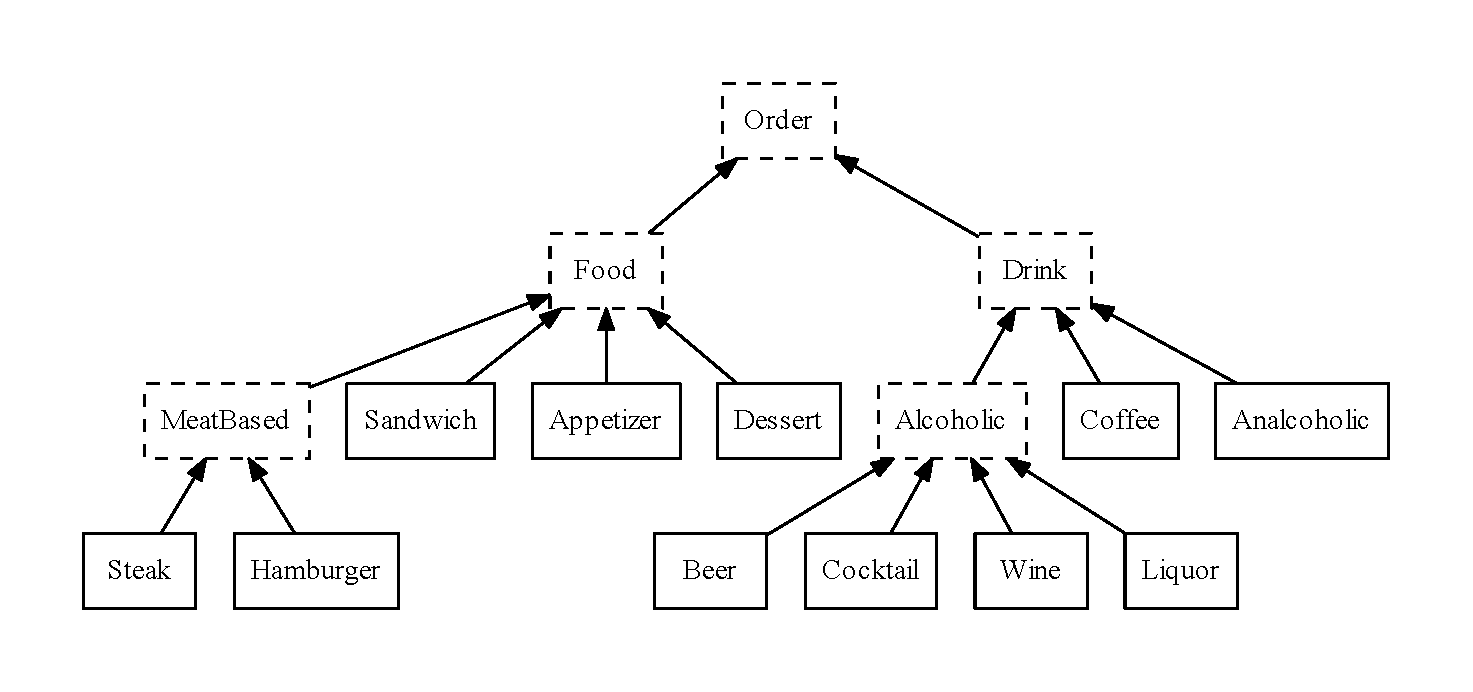
\includegraphics[width=\linewidth]{gerarchia.pdf}
\paragraph{Informazioni Generali} % (fold)
\label{par:informazioni_generali}
La gerarchia modella le ordinazioni inviate alla cucina del ristorante. Radicata nella classe polimorfa astratta \code{Order}, si dirama in due direzioni, \code{Food} e \code{Drink}, associate rispettivamente a ordinazioni di piatti e bevande. Il polimorfismo è dato da alcuni metodi virtuali, descritti in seguito, che forniscono funzionalità di copia e confronto polimorfi, e permettono di ricavare informazioni esplicite sul tipo degli oggetti. La gerarchia è fortemente estensibile sia "in orizzontale", aggiungendo nuovi sottotipi alle classi base presenti, sia "in verticale", fornendo sottotipi alle classi più derivate.
% paragraph informazioni_generali (end)
\paragraph{Membri Statici} % (fold)
\label{par:membri_statici}
La classe \code{Order} comprende anche dei membri statici, che forniscono due tipi di funzionalità:
\begin{itemize}
	\item Forniscono informazioni complessive sulla gerarchia.
	\item Forniscono informazioni e funzionalità relative ad un tipo a partire da una stringa.
\end{itemize}
In questo modo è possibile sfruttare una sorta di polimorfismo che non richiede un oggetto di invocazione.
% paragraph membri_statici (end)
\subsubsection{Order} % (fold)
\label{ssub:order}
\paragraph{Campi Dati} % (fold)
\label{par:campi_dati}
La classe \code{Order} incapsula informazioni di base relative ad un ordine attraverso tre campi dati privati di istanza:
\begin{itemize}
	\item \code{table}, il numero del tavolo,
	\item \code{item}, il nome della pietanza,
	\item \code{quantity}, il numero di porzioni
\end{itemize}
È presente un campo dati privato statico, \code{class_name}, che incapsula il nome della classe sottoforma di stringa. Sono inoltre presenti 4 metodi statici privati che permettono l'accesso a degli oggetti che, concettualmente, dovrebbero essere campi statici, ma per motivi progettuali (spiegati in seguito) sono allocati sullo heap e vengono acceduti attraverso puntatori di classe statica:
\begin{itemize}
	\item \code{static std::vector<std::string> &abstracts()}\newline
	Metodo che ritorna un \code{std::vector} contenente i nomi sottoforma di stringa delle classi astratte derivate da \code{Order}.
	\item \code{static std::vector<std::string> &types()}\newline
	Metodo che ritorna un \code{std::vector} contenente i nomi sottoforma di stringa delle classi istanziabili derivate da \code{Order}.
	\item \code{static std::multimap<std::string, std::pair<DetailType, std::string>> &info()}\newline
	Metodo che ritorna una \code{std::multimap} che associa a ciascun tipo derivato da \code{Order} la forma ed il nome dei dettagli specifici per quel tipo.
	\item \code{static std::map<std::string, std::function<DeepPtr<Order>(unsigned int,}\newline
	\code{const std::string &, unsigned int, const std::vector<std::string> &)>> &make()}\newline
	Metodo che ritorna una \code{std::map} che associa a ciascun tipo derivato da \code{Order} una funzione che agisce da costruttore, ritornando un puntatore smart ad un nuovo oggetto.
\end{itemize}
% paragraph campi_dati (end)
\paragraph{Metodi} % (fold)
\label{par:metodi}
Per l'interazione con gli oggetti sono disponibili $13$ metodi pubblici di istanza (virtuali e non) che comprendono un costruttore ed il distruttore, a cui vanno aggiunti il costruttore di copia e l'operatore di assegnazione di copia standard forniti dal compilatore. I metodi di istanza sono:
\begin{itemize}
	\item \code{Order(unsigned int, const std::string &, unsigned int)}\newline
	Costruisce un oggetto inizializzando i campi dati al valore del rispettivo parametro, in ordine.
	\item \code{virtual ~Order() = default}\newline
	Distruttore di default, dichiarato virtuale.
	\item \code{virtual Order *clone() const = 0}\newline
	Metodo di copia "standard", dichiarato virtuale puro per permettere la costruzione di copia polimorfa.
	\item \code{unsigned int getTable() const}\newline
	Getter per il campo dati \code{table}.
	\item \code{std::string getItem() const}\newline
	Getter per il campo dati \code{item}.
	\item \code{unsigned int getQuantity() const}\newline
	Getter per il campo dati \code{quantity}.
	\item \code{void setQuantity(unsigned int)}\newline
	Setter per il campo dati \code{quantity}.
	\item \code{virtual std::string getClassName() const}\newline
	Metodo virtuale che ritorna il nome della classe sottoforma di stringa.
	\item \code{virtual bool isA(const std::string &) const}\newline
	Metodo virtuale il cui parametro, \code{type}, è interpretato come il nome di una classe \code{Type}, e ritorna true se e solo se il tipo dinamico di \code{*this} è un sottotipo di \code{Type}.
	\item \code{virtual std::vector<std::string> getDetails() const = 0}\newline
	Metodo virtuale puro che ritorna un elenco di "dettagli" relativi all'ordine, cioè informazioni aggiuntive specifiche associate al tipo di pietanza ordinata.
	\item \code{virtual void setDetails(const std::vector<std::string> &) = 0}\newline
	Metodo virtuale puro speculare a \code{getDetails()}, permette di modificare le informazioni aggiuntive.
	\item \code{virtual bool operator==(const Order &) const}\newline
	Operatore di uguaglianza, dichiarato virtuale per tenere in considerazione dei dettagli relativi alle sottoclassi. L'implementazione "parziale" fornita da \code{Order} confronta i rispettivi tipi e i campi dati.
	\item \code{bool operator!=(const Order &) const}\newline
	Operatore di disuguaglianza, dichiarato non virtuale in quanto si basa sull'operatore di uguaglianza. Ritorna \code{true} se e solo se l'operatore di uguaglianza ritorna \code{false}.
\end{itemize}
Sono inoltre presenti 4 metodi pubblici statici che agiscono da getter per i "campi dati statici" allocati sullo heap:
\begin{itemize}
	\item \code{static const std::vector<std::string> &getAbstracts();}\newline
	Getter per \code{abstracts()}.
	\item \code{static const std::vector<std::string> &getTypes();}\newline
	Getter per \code{types()}.
	\item \code{static const std::multimap<std::string, std::pair<DetailType, std::string>> &getInfo();}\newline
	Getter per \code{info()}.
	\item \code{static const std::map<std::string, std::function<DeepPtr<Order>(unsigned int,}\newline
	\code{const std::string &, unsigned int, const std::vector<std::string> &)>> &getMake();}\newline
	Getter per \code{make()}.
\end{itemize}
% paragraph metodi (end)
\paragraph{Classi Annidate} % (fold)
\label{par:classi_annidate}
È presente una classe annidata protetta, \code{Empty}, la quale non ha campi dati, ed ha due costruttori:
\begin{itemize}
 	\item \code{Empty(const std::string &);}\newline
 	Il parametro viene interpretato come il nome di una classe astratta derivata da \code{Order}, e viene aggiunto a \code{abstracts()}.
	\item \code{Empty(const std::string &, const std::vector<std::pair<DetailType, std::string>> &,}\newline
	\code{const std::function<DeepPtr<Order>(unsigned int, const std::string &, unsigned int,}\newline
	\code{const std::vector<std::string> &)> &);}\newline
	Il primo parametro, \code{type}, viene interpretato come il nome di un tipo derivato da \code{Order}, e viene aggiunto a \code{types()}; il secondo, \code{details}, come un elenco di coppie (forma, nome) associate a dettagli di una classe derivata, e quindi ogni suo elemento viene agiunto a \code{info()} utilizzando \code{type} come chiave; infine, il terzo parametro, \code{constructor}, viene interpretato come una funzione che agisce da costruttore, e quindi viene aggiunto a \code{make()} utilizzando ancora \code{type} come chiave.
\end{itemize}
È inoltre presente una scoped enumeration, \code{DetailType}, che rappresenta le varie forme che possono assumere i dettagli aggiunti dalle classi derivate:
\begin{itemize}
	\item \code{DetailType::Choice}, una scelta fra due alternative.
	\item \code{DetailType::SmallText}, un breve testo (ad esempio una dimensione, o una temperatura).
	\item \code{DetailType::LargeText}, un testo più lungo (ad esempio una descrizione o un elenco).
\end{itemize}
% paragraph classi_annidate (end)
\paragraph{"Polimorfismo su Stringhe"} % (fold)
\label{par:_polimorfismo_su_stringhe_}
Per assicurare il corretto popolamento di \code{abstracts()}, \code{types()}, \code{info()}, e \code{make()} è necessario che ciascuna classe derivata (anche indirettamente) da \code{Order} abbia un campo dati statico, possibilimente privato, di tipo \code{Empty}, e che esso sia inizializzato con il costruttore adeguato: per le classi astratte quello ad un parametro, a cui va passato il nome della classe, mentre per le classi istanziabili quello a tre parametri, a cui vanno passati il nome della classe, l'elenco dei dettagli, come coppie (forma, nome), e una funzione che agisca da costruttore. In particolare, i dettagli nell'elenco devono essere nello stesso ordine in cui vengono ritornati dal metodo \code{getDetails()}. Questo sistema garantisce che i 4 container siano popolati correttamente all'avvio dell'applicazione grazie al fatto che i campi dati statici sono costruiti prima dell'esecuzione della funzione \code{main()}, ed essendo completamente automatico esonera l'utente della gerarchia dall'invocazione di un'ipotetica funzione \code{setup()}. Il tutto si basa sulla garanzia che i 4 container siano costruiti prima di essere popolati, ed è per questo che vengono costruiti sullo heap ed acceduti attraverso puntatori di classe statica locali ai metodi di accesso: essendo di classe statica, le inizializzazioni dei puntatori vengono eseguite solo una volta, la prima volta che le funzioni vengono invocate, cioè la prima volta che un campo statico di tipo \code{Empty} viene costruito. D'altro canto, essendo allocati sullo heap andrebbero deallocati con \code{delete}, cosa che non avviene, ma siccome andrebbero deallocati dopo l'esecuzione della \code{main} questo non consiste in un memory leak, perchè in questo momento la memoria viene comunque reclamata dal sistema operativo. 
% paragraph _polimorfismo_su_stringhe_ (end)
\paragraph{RTTI su stringhe} % (fold)
\label{par:rtti_su_stringhe}
I metodi \code{getClassName()} e \code{isA()} forniscono una versione basata su stringhe dei meccanismi di RTTI. Considerando una reference valida \code{o} di tipo \code{Order &} (oppure, per un ragionamento analogo, un puntatore valido di tipo \code{Order *}), l'invocazione \code{o.getClassName()} ritorna una stringa analoga a quella ritornata da \code{typeid(o).name()}, con la particolarità che la prima è fissata dal programmatore, mentre la seconda è implementation defined. In modo simile, se \code{type} è una stringa contenente il nome di una classe \code{Type}, l'invocazione \code{o.isA(type)} è analoga a \code{dynamic_cast<Type *>(&o)!=nullptr}, ma in questo caso la differenza, più marcata, è che \code{isA()} "agisce" su stringhe, mentre il \code{dynamic_cast} "agisce" su tipi.
% paragraph rtti_su_stringhe (end)
% subsubsection order (end)
\subsubsection{Food} % (fold)
\label{ssub:food}
La classe astratta \code{Food}, derivata da \code{Order}, rappresenta ordini di piatti. Presenta un campo dati aggiuntivo \code{without}, dotato di getter e setter, che rappresenta parti del piatto che il cliente ha chiesto di escludere; per tenere in considerazione il nuovo campo dati è presente un costruttore adeguato. Il metodo \code{clone()}, pur rimanendo virtuale puro, subisce overriding per modificare il tipo di ritorno (che è quindi covariante). Gli altri metodi virtuali sono reimplementati come da aspettative.
% subsubsection food (end)
\subsubsection{MeatBased} % (fold)
\label{ssub:meatbased}
La classe astratta \code{MeatBased}, derivata da \code{Food}, rappresenta ordini di piatti il cui ingrediente principale è un tipo di carne, e per questo ha un ulteriore campo dati \code{temperature}, dotato di getter e setter, che rappresenta la temperatura di cottura della carne; è quindi fornito un costruttore adeguato. Il metodo \code{clone()} subisce ancora override, ma non viene ancora implementato. Gli altri metodi virtuali sono reimplementati come da aspettative.
% subsubsection meatbased (end)
\subsubsection{Steak, Hamburger} % (fold)
\label{ssub:steak_hamburger}
Le classi \code{Steak} e \code{Hamburger}, derivate da \code{MeatBased}, rappresentano ordini di piatti il cui ingrediente principale è rispettivamente una bistecca o un hamburger. Non presentano campi dati aggiuntivi, ma \code{Steak} non fa uso del campo dati \code{without} di \code{Food}; di conseguenza, \code{Hamburger} utilizza il costruttore di \code{MeatBased}, mentre \code{Steak} ne fornisce uno ad hoc. Per lo stesso motivo, solo \code{Steak} reimplementa \code{getDetails()}, \code{setDetails()} e l'operatore di uguaglianza. Gli altri metodi virtuali sono reimplementati come da aspettative.
% subsubsection steak_hamburger (end)
\subsubsection{Sandwich} % (fold)
\label{ssub:sandwich}
La classe \code{Sandwich}, derivata da \code{Food}, rappresenta ordini di piatti basati su sandwich. Non presenta campi dati aggiuntivi, e di conseguenza utilizza il costruttore di \code{Food}. Per lo stesso motivo, non reimplementa \code{getDetails()}, \code{setDetails()} e l'operatore di uguaglianza. Gli altri metodi virtuali sono reimplementati come da aspettative.
% subsubsection sandwich (end)
\subsubsection{Appetizer, Dessert} % (fold)
\label{ssub:appetizer_e_dessert}
Le classi \code{Appetizer} e \code{Dessert}, derivate da \code{Food}, rappresentano ordini di antipasti e dolci, rispettivamente. Ciascuna ha un campo dati aggiuntivo, \code{sauces} e \code{with} nell'ordine, con getter e setter, ed entrambe non fanno uso del campo dati \code{without} di \code{Food}. Per questo forniscono entrambe costruttori, ed entrambe reimplementano \code{getDetails()}, \code{setDetails()} e l'operatore di uguaglianza. Gli altri metodi virtuali sono reimplementati come da aspettative.
% subsubsection appetizer_e_dessert (end)
\subsubsection{Drink} % (fold)
\label{ssub:drink}
La classe astratta \code{Drink}, derivata da \code{Order}, rappresenta ordini di bevande; non presenta nessun campo dati aggiuntivo, e quindi utilizza il costruttore di \code{Order}. Il metodo \code{clone()}, subisce overriding per modificare il tipo di ritorno ma non viene implementato, come non vengono implementati \code{getDetails()}, \code{setDetails()} e l'operatore di uguaglianza. Gli altri metodi virtuali sono reimplementati come da aspettative.
% subsubsection drink (end)
\subsubsection{Alcoholic} % (fold)
\label{ssub:alcoholic}
La classe astratta \code{Alcoholic}, derivata da \code{Drink}, rappresenta ordini di bevande alcoliche; non presenta nessun campo dati aggiuntivo, e quindi utilizza il costruttore di \code{Drink}. Il metodo \code{clone()}, subisce overriding per modificare il tipo di ritorno ma non viene implementato, come non vengono implementati \code{getDetails()}, \code{setDetails()} e l'operatore di uguaglianza. Gli altri metodi virtuali sono reimplementati come da aspettative.
% subsubsection alcoholic (end)
\subsubsection{Beer, Cocktail, Wine, Liquor} % (fold)
\label{ssub:beer_cocktail_wine_liquor}
Le classi \code{Beer}, \code{Cocktail}, \code{Wine}, e \code{Liquor}, derivate da \code{Alcoholic}, rappresentano ordini di birre, cocktail, vini, e liquori, rispettivamente. Ciascuna ha un campo dati aggiuntivo, \code{size}, \code{garnish}, \code{vintage} e \code{ice} nell'ordine, con getter e setter, e per questo forniscono tutte costruttori. I metodi virtuali sono reimplementati come da aspettative.
% subsubsection beer_cocktail_wine_liquor (end)
\subsubsection{Coffee, Analcoholic} % (fold)
\label{ssub:coffe_analcoholic}
Le classi \code{Coffee} e \code{Analcoholic}, derivate da \code{Drink}, rappresentano ordini di caffè e bibite analcoliche, rispettivamente. Ciascuna ha un campo dati aggiuntivo, \code{notes} e \code{ice} nell'ordine, con getter e setter, e per questo forniscono entrambe costruttori. I metodi virtuali sono reimplementati come da aspettative.
% subsubsection coffe_analcoholic (end)
% subsection gerarchia_di_tipi (end)
\subsection{Template Container} % (fold)
\label{sub:template_container}
Le istanze del template di classe \code{Container<T>} sono contenitori che permettono di gestire collezioni di oggetti polimorfi (in caso non lo siano il template è comunque istanziabile, ma è necessario fornire specializzazioni ai template di funzione contenuti nel namespace \code{UniformInterface}, e il contenitore risultante è inutilmente appesantito). Siccome l'applicazione richiede che si possano eseguire inserimenti e rimozioni in posizione arbitraria nel container, si è scelto in fase di progettazione di utilizzare una lista doppiamente concatenata; si è inoltre scelto di fornire un'interfaccia pubblica il più simile possibile a quella del template \code{std::list<T>}.
\subsubsection{Classi annidate} % (fold)
\label{ssub:classi_annidate}
Essendo una lista concatenata, il template di classe si appoggia su un template di struttura annidata \code{Node}, che presenta diversi costruttori adatti ai diversi modi di passare gli oggetti da aggiungere al container come parametri, il distruttore, ed un overloading per l'operatore di uguaglianza, che esegue il confronto fra i campi info dei nodi considerati, e anche dei successivi. Sono inoltre forniti due template di classe annidati \code{iterator<T>} e \code{const_iterator<T>}; in realtà, questi sono specializzazioni parziali del template di classe annidata \code{temp_iterator<T,bool>}, il cui parametro non-tipo è \code{true} per \code{const_iterator<T>} e \code{false} per \code{iterator<T>}. Questo, combinato con i template \code{reference<T,bool>} e \code{pointer<T,bool>} contenuti nel namespace \code{ReferenceTypes}, permette di evitare definire due classi separate, ma fortemente accoppiate, per gli iteratori e gli iteratori costanti, al costo di non permettere il cast da \code{iterator<T>} a \code{const_iterator<T>}. È fornito un costruttore privato ad un parametro, e per questo il template \code{Container} è dichiarato come template di classe friend associato, mentre il costruttore di default (che costruisce un iteratore non dereferenziabile) è pubblico; inoltre, sono presenti (e pubblici) i costruttori di copia e di move forniti dal compilatore, come anche i rispettivi operatori di assegnazione e il distruttore. Gli iteratori forniscono overloading per gli operatori di dereferenziazione, dereferenziazione e selezione, incremento e decremento prefisso e postfisso, e confronto. Il confronto è superficiale: l'operatore di uguaglianza ritorna \code{true} se e solo se i due iteratori puntano allo stesso nodo. In caso di comportamenti anomali, i metodi lanciano delle appropriate eccezioni.
% subsubsection classi_annidate (end)
\subsubsection{Metodi} % (fold)
\label{ssub:metodi}
\paragraph{Costruttori, Distuttore, Assegnazione} % (fold)
\label{par:costruttori_distuttore_assegnazione}
Il container fornisce 6 costruttori, di cui due sono il costruttore di copia e quello di move, i quali sono accompagnati dal distruttore e dagli operatori di assegnazione di copia e di move per la rule of five, che dallo standard C++11 ha sostituito la rule of three. I rimanenti costruttori permettono di costruire un container vuoto, un container di una data dimensione con nodi tutti uguali, un container a partire da un range, oppure un container a partire da una initializer list.
% paragraph costruttori_distuttore_assegnazione (end)
\paragraph{Iterazione} % (fold)
\label{par:iterazione}
Per l'iterazione sono forniti 6 metodi, completamente analoghi ai metodi \code{begin()}, \code{begin() const}, \code{cbegin() const}, \code{end()}, \code{end() const} e \code{cend() const} forniti dai container della STL. È inoltre fornito un metodo statico \code{toConstIter()} per convertire da \code{iterator<T>} a \code{const_iterator<T>}.
% paragraph iterazione (end)
\paragraph{Dimensione, Accesso, Inserimento, Rimozione} % (fold)
\label{par:dimensione_accesso_inserimento_rimozione}
Sono forniti un metodo \code{size()} che ritorna la dimensione della lista, e un metodo \code{empty()} che ritorna \code{true} se e solo se la lista è vuota, e metodi \code{front()} e \code{back()} \code{const} e non, per l'accesso al primo e all'ultimo elemento. Sono forniti metodi \code{push_back()}, \code{push_front()}, \code{pop_back()}, e \code{pop_front()} per l'inserimento e la rimozione in testa e in coda alla lista (ciascuno dotato di diversi overloading),ed inoltre metodi \code{insert()} ed \code{erase()} per l'inserimento e la rimozione in posizione arbitraria, basati su iteratori. È fornito un metodo \code{clear()} per svuotare il container. Infine, sono forniti metodi \code{swap()} (in due versioni, per scambiare il contenuto di due container o di due nodi) e \code{give} (per spostare un nodo da un container ad un altro, o da un punto ad un altro nello stesso container);
% paragraph dimensione_accesso_inserimento_rimozione (end)
\paragraph{Ricerca, Confronto} % (fold)
\label{par:ricerca_confronto}
Sono forniti metodi \code{find()} e \code{find_if}, \code{const} e non, per la ricerca di elementi nel container (\code{find()} utilizza l'operatore di confronto fornito da \code{DeepPtr<T>}, mentre \code{find_if()} utilizza una funzione passata come parametro, la quale deve avere due parametri di tipo \code{const T &} e tipo di ritorno \code{bool}). Sono forniti inoltre operatori di confronto; l'operatore di uguaglianza ritorna \code{true} se e solo se i due container hanno gli stessi elementi nello stesso ordine.
% paragraph ricerca_confronto (end)
% subsubsection metodi (end)
% subsection template_container (end)
\subsection{Altre Classi} % (fold)
\label{sub:altre_classi}
Oltre alla gerarchia radicata in \code{Order} e al template \code{Container}, sono state definite altre classi.
\subsubsection{Template DeepPtr} % (fold)
\label{ssub:template_deepptr}
Il template di classe \code{DeepPtr<T>} è un template per puntatori smart. Gli oggetti delle classi istanziate da questo template utilizzano un campo dati di tipo \code{T *} per la gestione di oggetti anche polimorfi. La gestione profonda della memoria è garantita grazie a costruttore di copia, costruttore di move, operatore di assegnazione di copia, operatore di assegnazione di move, e distruttore. I rimanenti costruttori generano puntatori smart ad una copia dell'oggetto passato come parametro. Sono forniti operatori di dereferenziazione e di dereferenziazione e selezione, ciascuno in due versioni, \code{const} e non-\code{const}, ed operatori di confronto, che eseguono il confronto fra gli oggetti puntati. Sono inoltre forniti i metodi \code{swap()}, per scambiare i contenuti di due puntatori smart, e \code{takeResponsibility()}, per associare il puntatore smart ad un oggetto preesistente, invece di costruirne uno di copia. Per la copia e il confronto vengono utilizzati dei template di funzione contenuti nel namespace \code{UniformInterface}, che nella loro versione di default chiamano un metodo \code{clone()} e l'operatore di uguaglianza, ma che in caso di tipi privi di questi metodi permettono di essere adattati attraverso la specializzazione.
% subsubsection template_deepptr (end)
\subsubsection{Eccezioni} % (fold)
\label{ssub:eccezioni}
Sono state definite le classi \code{EmptyContainer}, \code{InvalidFile}, \code{InvalidIterator}, \code{NullPrtExcept}, e \code{UnavailableFile} per sollevare eccezioni. \code{InvalidFile} e \code{UnavailableFile} derivano da \code{std::invalid_argument}, mentre le restanti derivano da \code{std::logic_error}. Comunque tutte le classi sono parte della gerarchia radicata in \code{std::exception}.
% subsubsection eccezioni (end)
\subsubsection{Finestre di Dialogo} % (fold)
\label{ssub:finestre_di_dialogo}
Le classi \code{AddOrderDialog}, \code{EditOrderDialog}, e \code{SearchDialog} forniscono all'utente della GUI la possibilità di inserire informazioni, nello specifico per inserire nuovi ordini, modificare ordini esistenti, e selezionare ordini che rispettano specifiche caratteristiche. Sono tutte derivate da \code{QDialog}, in modo da rendere modali le finestre associate ai rispettivi oggetti. Tutte sfruttano \code{Order::info()} per rappresentare i dettagli specifici del tipo selezionato nel modo appropriato. In \code{AddOrderDialog} e \code{EditOrderDialog} le informazioni inserite dall'utente sono comunicate all'applicazione attraverso dei metodi essenzialmente analoghi a dei getter, mentre \code{SearchDialog} sfrutta due getter per comunicare se includere gli ordini in attesa e/o quelli completati, ed un metodo che ritorna un oggetto di tipo \code{std::function} che racchiude un predicato ad un parametro di tipo \code{const Order &} e ritorna \code{true} se e solo se il parametro rispetta le condizioni inserite dall'utente.
% subsubsection finestre_di_dialogo (end)
\subsubsection{OrderWidget} % (fold)
\label{ssub:orderwidget}
La classe \code{OrderWidget}, derivata da \code{QFrame}, permette di rappresentare gli ordini nella GUI. Contiene dei pulsanti che permettono all'utente di modificare l'ordine, completarlo o rimuoverlo, e sfrutta dei segnali per comunicare queste informazioni al resto dell'applicazione. Ogni oggetto di tipo \code{OrderWidget} contiene un indice (cioè un campo dati di tipo \code{Model::Index}, descritto in seguito) che punta al corrispettivo ordine. Come le finestre di dialogo, la classe sfrutta \code{Order::info()} per rappresentare i dettagli specifici dell'ordine nel modo appropriato. Ogni \code{OrderWidget} mostra un'icona appropriata al tipo dell'ordine associato, ed in caso di estensione della gerarchia è necessario aggiungere le icone necessarie attraverso il resource system di Qt. In particolare, l'immagine relativa al tipo \code{example} deve essere accessibile attraverso il prefisso \code{/type} e l'alias \code{example}: il path completo, indipendentemente dal nome del file, deve essere \code{:/type/example}.
% subsubsection orderwidget (end)
\subsubsection{Model, View, SearchView} % (fold)
\label{ssub:model_view_searchview}
Le classi \code{Model} e \code{View} costituiscono il fulcro dell'applicazione. \code{Model} racchiude la logica del programma, gestisce i due container di ordini in attesa e completati, permette di aggiungere ordini, rimuoverli, spostarli da un container all'altro, salvare su file e caricare da file, cercare all'interno dei due container ordini che rispettano certe caratteristiche, e ottenere l'elenco degli ordini incompleti. Espone il tipo \code{Model::Index}, che coincide con il tipo iteratore di \code{Container<Order>}, per permettere alla GUI di mantenere un collegamento diretto con gli ordini. \code{View}, classe derivata da \code{QMainWindow}, rappresenta la finestra principale dell'applicazione. È dotata di una toolbar per le operazioni eseguibili, ed utilizza una \code{QScrollArea} per visualizzare l'elenco degli ordini, ciascuno rappresentato da un \code{OrderWidget}. La classe \code{SearchView}, derivata da \code{QDialog} perchè sia modale, permette di visualizzare l'elenco degli ordini risultante da una ricerca. Inoltre, permette di rimuoverli o completarli tutti, chiedendo conferma all'utente attraverso un message box.
% subsubsection model_view_searchview (end)
% subsection altre_classi (end)
\subsection{Chiamate polimorfe} % (fold)
\label{sub:chiamate_polimorfe}

% subsection chiamate_polimorfe (end)
\subsection{Formato dei file di salvataggio e caricamento} % (fold)
\label{sub:formato_dei_file_di_salvataggio_e_caricamento}

% subsection formato_dei_file_di_salvataggio_e_caricamento (end)
% section descrizione_aspetti_progettuali (end)
\section{Note tecniche} % (fold)
\label{sec:note_tecniche}
\subsection{Istruzioni di compilazione} % (fold)
\label{sub:istruzioni_di_compilazione}
Per la compilazione è fornito il file \code{progetto.pro}.
% subsection istruzioni_di_compilazione (end)
\subsection{Ambiente di sviluppo} % (fold)
\label{sub:ambiente_di_sviluppo}
\begin{itemize}
	\item Sistema operativo di sviluppo: Windows 10 Home 64-bit
	\item Compilatore: g++ (i686-posix-dwarf-rev0, Built by MinGW-W64 project) 5.3.0
	\item Qt framework: Qt 5.12.0
	\item IDE di sviluppo: Qt Creator 4.8.1
\end{itemize}
% subsection ambiente_di_sviluppo (end)
\subsection{Ripartizione ore} % (fold)
\label{sub:ripartizione_ore}
\begin{itemize}
	\item Analisi preliminare del problema: 1
	\item Progettazione modello: 1
	\begin{itemize}
		\item Progettazione template di classe \code{Container}: 0.5
		\item Progettazione gerarchia di classi: 1.5
	\end{itemize}
	\item Progettazione GUI: 1 (per ora)
	\item Apprendimento libreria Qt: 15 (da specificare, esterne alle ore del progetto, scrivi che hai smanettato per un altro progetto)
	\item Codifica modello: 17
	\begin{itemize}
		\item Codifica template di classe \code{Container}: 8
		\item Codifica gerarchia di classi: 9
	\end{itemize}
	\item Codifica GUI: (4) per ora
	\item Debugging
	\item Testing
\end{itemize}
% subsection ripartizione_ore (end)
% section note_tecniche (end)
\end{document}